\documentclass[presentation]{beamer}

\usepackage{tikz}
\usetikzlibrary{positioning,calc,matrix}
\usetikzlibrary{shapes.geometric}
\usetikzlibrary{backgrounds}% only to show the bounding box
\usepackage{pgf}
\usepackage{appendixnumberbeamer}
\usepackage{amsmath}
\DeclareMathOperator{\tr}{tr}
\date{6th July 2017}
\usetheme{metropolis}
\metroset{progressbar=frametitle}

\renewcommand{\vec}[1]{\ensuremath{\boldsymbol{#1}}}
\newcommand{\ddt}[1]{\frac{\partial #1}{\partial t}}
\newcommand{\zhat}{\hat{\vec{z}}}
\newcommand{\W}{\ensuremath{\mathbb{W}}}

\newcommand{\inner}[1]{\left\langle #1 \right \rangle}

\newcommand{\KSP}[2]{\ensuremath{\mathcal{K}\left(#1, \mathbb{#2}\right)}}
\newcommand{\ksp}[1]{\KSP{#1}{#1}}

\newcommand{\highlight}[1]{\colorbox{red!20}{\color{black} #1}}
\newcommand{\arxivlink}[2]{%
  \href{http://www.arxiv.org/abs/#1}%
  {{\small\texttt{arXiv:\,#1\,[#2]}}}%
}
\newcommand{\doilink}[1]{%
  \href{http://dx.doi.org/#1}%
  {{\small\texttt{doi:\,#1}{}}}%
}

\author{Lawrence Mitchell\inst{1,*}}
\institute{
\inst{1}Departments of Computing and Mathematics, Imperial College
London

\inst{*}\texttt{lawrence.mitchell@imperial.ac.uk}
}

\graphicspath{{./\jobname.figures/}}

\usepackage[url=false,
            doi=true,
            isbn=false,
            style=authoryear,
            firstinits=true,
            uniquename=init,
            backend=biber]{biblatex}

\setbeamertemplate{bibliography item}{}

\renewcommand{\bibfont}{\footnotesize}
\addbibresource{references.bib}

\setlength{\bibitemsep}{1ex}
\setlength{\fboxsep}{1pt}

\renewbibmacro{in:}{}
\DeclareFieldFormat[article]{volume}{\textbf{#1}}
\DeclareFieldFormat{doi}{%
  doi\addcolon%
  {\scriptsize\ifhyperref{\href{http://dx.doi.org/#1}{\nolinkurl{#1}}}
    {\nolinkurl{#1}}}}
\AtEveryBibitem{%
\clearfield{pages}%
\clearfield{issue}%
\clearfield{number}%
}

\usepackage{minted}
\RecustomVerbatimEnvironment{Verbatim}{BVerbatim}{}

\title{Firedrake: symbolic numerical computing}
\begin{document}
\maketitle

% \setbeamertemplate{background}{}
% \setbeamercolor{footline}{
%   use=normal text,
%   fg=normal text.fg,
% }

\section{Introduction}
\begin{frame}
  \frametitle{Finite element crash course}
  \begin{align*}
    F(u) &= 0 \text{ in $\Omega$}\\
    u &= g \text{ on $\Gamma_1$}\\
    \frac{\partial u}{\partial n} &= h \text{ on $\Gamma_2$}
  \end{align*}
  Seek \emph{weak} solution in some space of functions $V(\Omega)$.

  Now we need to solve the (infinite dimensional) problem, find $u\in V$ s.t.
  \begin{equation*}
    \int_\Omega \!F(u) v\, \text{d}x = 0 \quad \forall\, v \in V
  \end{equation*}
\end{frame}
\begin{frame}
  \frametitle{Finite element crash course}
  Choose finite dimensional $V_h \subset V$, and seek a solution in
  that subspace: find $u_h \in V_h$ s.t.
  \begin{equation*}
    \int_\Omega \!F(u_h) v_h\, \text{d}x = 0 \quad \forall\, v_h \in V_h
  \end{equation*}
\end{frame}
\begin{frame}
  \frametitle{Finite element crash course}
  \begin{overprint}
    \only<1>{Divide domain $\Omega$\dots
    \begin{center}
      \begin{tikzpicture}
        \draw[very thick, line cap=rect] (0,0) -- (5, 0) (0, 0) arc
        (180:360:2.5);
      \end{tikzpicture}
    \end{center}}
  \only<2>{\dots{}into triangulation $\mathcal{T}$\dots
    \begin{center}
        \begin{tikzpicture}
          \path (0,0) arc[radius=2.5, start angle=180, end angle=360]
          node[name=E,pos=0,swap] {} node[name=F,pos=0.25,swap] {}
          node[name=G,pos=0.5,swap] {} node[name=H,pos=0.82,swap] {}
          node[name=I,pos=1,swap] {}; \node (A) at (2.5, 0) {}; \node
          (B) at (1.4, -0.7) {}; \node (C) at (3.4, -1.2) {}; \node
          (D) at (1.8, -1.5) {};

          \draw[color=black, very thick, line cap=butt, line
          join=round] (E.center) -- (A.center) -- (I.center) --
          (H.center) -- (G.center) -- (F.center) -- (E.center) --
          cycle; \draw[color=black, very thick, line cap=butt, line
          join=round] (E.center) -- (B.center) -- (D.center) --
          (F.center) -- (B.center); \draw[color=black, very thick,
          line cap=butt, line join=round] (G.center) -- (D.center) --
          (C.center) -- (G.center); \draw[color=black, very thick,
          line cap=butt, line join=round] (B.center) -- (A.center) --
          (C.center) -- (B.center); \draw[color=black, very thick,
          line cap=butt, line join=round] (H.center) -- (C.center) --
          (I.center);
        \end{tikzpicture}
    \end{center}
  }
  \only<3>{\dots{}and choose basis with finite support.
    \begin{center}
        \begin{tikzpicture}
          \path (0,0) arc[radius=2.5, start angle=180, end angle=360]
          node[name=E,pos=0,swap] {} node[name=F,pos=0.25,swap] {}
          node[name=G,pos=0.5,swap] {} node[name=H,pos=0.82,swap] {}
          node[name=I,pos=1,swap] {}; \node (A) at (2.5, 0) {}; \node
          (B) at (1.4, -0.7) {}; \node (C) at (3.4, -1.2) {}; \node
          (D) at (1.8, -1.5) {};

        \path[fill=gray!50] (E.center) -- (A.center) -- (B.center) --
        (F.center) --cycle;
          \draw[color=black, very thick, line cap=butt, line
          join=round] (E.center) -- (A.center) -- (I.center) --
          (H.center) -- (G.center) -- (F.center) -- (E.center) --
          cycle; \draw[color=black, very thick, line cap=butt, line
          join=round] (E.center) -- (B.center) -- (D.center) --
          (F.center) -- (B.center); \draw[color=black, very thick,
          line cap=butt, line join=round] (G.center) -- (D.center) --
          (C.center) -- (G.center); \draw[color=black, very thick,
          line cap=butt, line join=round] (B.center) -- (A.center) --
          (C.center) -- (B.center); \draw[color=black, very thick,
          line cap=butt, line join=round] (H.center) -- (C.center) --
          (I.center);
        \end{tikzpicture}
      \end{center}
      }
  \end{overprint}
\end{frame}

\begin{frame}
  \frametitle{Finite element crash course}
  Integrals become sum over element integrals
  \begin{equation*}
    \int_\Omega\! F(u_h) v_h \, \text{d}x =
    \sum_{e \in \mathcal{T}} \int_e\! F(u_h)v_h\, \text{d}x
  \end{equation*}

  (Usually) perform element integrals with numerical quadrature
  \begin{equation*}
    \int_e F(u_h)v_h\,\text{d}x = \sum_q w_q F(u_h(q)) v_h(q)
  \end{equation*}

  Replace $u_h(q), v_h(q)$ with expansion in finite element basis
  \begin{align*}
    u_h(q) &= \sum_i u_h^i \phi_i(q)\\
    v_h(q) &= \phi_j(q)\\
  \end{align*}
\end{frame}

\begin{frame}
  \frametitle{Abstractly}
  \begin{itemize}
  \item Mathematics says ``here is the integral to compute on each
    element, do that everywhere''
  \item Doesn't specify \emph{how} to compute the integral
  \item Doesn't specify \emph{how} to gather the element contributions
  \end{itemize}
\end{frame}

\begin{frame}[fragile]
  \frametitle{Mechanical translation}
  \begin{block}{Assertion}
    Once we pick the discretisation, writing the code for $\sum_q w_q
    F(u_h(q)) v_h(q)$ is mechanical.
  \end{block}
  \begin{center}
    \begin{overlayarea}{\textwidth}{0.8\textheight}
      \begin{onlyenv}<1>
\begin{minted}[fontsize=\tiny]{cpp}
template<typename EG, typename LFSU, typename X, typename LFSV, typename M>
void jacobian_volume(const EG& eg, const LFSU& lfsu, const X& x,
                     const LFSV& lfsv, M& mat) const {
  const auto geo = eg.geometry();
  const auto S = geo.jacobianInverseTransposed(qp);
  RF factor = weight*geo.integrationElement(qp);
  double grad[dim][n] = {{0.0}};
  for (int i=0; i<dim; i++)
    for (int k=0; k<dim; k++)
      for (int j=0; j<n; j++)
        grad[i][j] += S[i][k] * gradhat[k][j];
  double A[n][n] = {{0.0}};
  for (int i=0; i<n; i++)
    for (int k=0; k<dim; k++)
      for (int j=0; j<n; j++)
        A[i][j] += grad[k][i]*grad[k][j];
  for (int i=0; i<n; i++)
    for (int j=0; j<n; j++)
      mat.accumulate(lfsu,i,lfsu,j,A[i][j]*factor);
}
\end{minted}
      \end{onlyenv}
      \begin{onlyenv}<2>
        \begin{equation*}
          \int_\Omega \nabla u \cdot \nabla v\,\text{d}x
        \end{equation*}
      \end{onlyenv}
      \begin{onlyenv}<3>
        \begin{corollary}
          Computers are good at mechanical things, why don't we get the
          computer to write the element integral?
        \end{corollary}
      \end{onlyenv}
    \end{overlayarea}
\end{center}
\end{frame}
\begin{frame}
  \frametitle{Firedrake}

  An automated finite element system.

  \begin{center}
    \url{www.firedrakeproject.org}\\
  \end{center}

  \begin{flushright}
    {\footnotesize F. Rathgeber, D.A. Ham, \textbf{LM}, M. Lange,
      F. Luporini, A.T.T. McRae, G.-T. Bercea, G.R. Markall,
      P.H.J. Kelly. ACM Transactions on Mathematical Software,
      2016. \arxivlink{1501.01809}{cs.MS}}
  \end{flushright}
\end{frame}

\begin{frame}
  \frametitle{Exploiting abstractions}
  \begin{itemize}
  \item Firedrake builds on, and extends, embedded DSLs developed in
    the FEniCS project \url{www.fenicsproject.org}
  \item The \emph{Unified Form Language} \parencite{Alnaes:2014} to
    specify variational forms
  \item A symbolic problem description (generic) is woven together with
    problem-specific data, and executed by a runtime Python library
    that does JIT code compilation.
  \end{itemize}
\end{frame}
\begin{frame}[fragile]
  \frametitle{UFL: a DSL for variational problems}
  \begin{equation*}
    \int_\Omega \nabla u \cdot \nabla v\,\text{d}x
  \end{equation*}

\begin{minted}[fontsize=\scriptsize]{python}
V = FiniteElement("Lagrange", triangle, 1)
u = TrialFunction(V)
v = TestFunction(V)
a = dot(grad(u), grad(v))*dx
\end{minted}
\end{frame}

\begin{frame}[fragile]
  \frametitle{Not just toy models}
  \begin{columns}
    \begin{column}{0.4\textwidth}
      \begin{align*}
        \mathbf{F} &= \mathbf{I} + \nabla \mathbf{u}\\
        \mathbf{C} &= \mathbf{F}^T \mathbf{F}\\
        \mathbf{E} &= (\mathbf{C} - \mathbf{I}) / 2\\
        \Psi &= \frac{\lambda}{2}[\tr(\mathbf{E})]^2 + \mu \tr(\mathbf{E}^2)\\
        \mathbf{S} &= \frac{\partial \Psi}{\partial \mathbf{E}}\\
        \mathbf{P} &= \mathbf{F} \mathbf{S}\\
        r &= \int_\Omega \mathbf{P} : \nabla \mathbf{v} - \mathbf{b} \cdot \mathbf{v}\,\text{d}x\\
        a &= \lim_{\epsilon \to 0} \frac{r(\mathbf{u} + \epsilon \delta \mathbf{u}) - r(\mathbf{u})}{\epsilon}
      \end{align*}
    \end{column}
    \begin{column}{0.6\textwidth}
\begin{minted}[fontsize=\tiny]{python}
V = VectorElement("Lagrange", triangle, 2)
v = TestFunction(V)
du = TrialFunction(V) # Incremental displacement
u = Coefficient(V)    # Displacement
B = Coefficient(V)    # Body force per unit mass
I = Identity(V.cell().topological_dimension())
F = I+grad(u)  # Deformation gradient
C = F.T*F      # Right Cauchy-Green tensor
E = (C - I)/2
E = variable(E)
# Material constants
mu = Constant(triangle)
lmbda = Constant(triangle)
# Strain energy function (material model)
psi = lmbda/2*(tr(E)**2) + mu*tr(E*E)
S = diff(psi, E) # Second Piola-Kirchhoff stress tensor
P = F*S          # First Piola-Kirchoff stress tensor
# Variational problem
r = (inner(PK, grad(v)) - inner(B, v))*dx
a = derivative(r, u, du)
\end{minted}
    \end{column}
  \end{columns}
\end{frame}

- We make progress in science by building on the work of others

- Sophisticated reasoning about complex algorithms in computational
science is possible due to creation of appropriate abstractions.

- Yet often, these abstractions are not mirrored in the computational
implementation

- Status quo

- Multigrid solver

- Solver composition


\section{Lecture excerpt}

\begin{frame}[fragile]
  \frametitle{Pitfalls when computing with numbers}
  \begin{itemize}
  \item Computers are an excellent way to build models of the physical
    world.
  \item But we have to be careful to remember that computer arithmetic
    does not behave the same as mathematics.
  \item We'll look at some examples from integer and real arithmetic
  \end{itemize}
\end{frame}

\begin{frame}[plain,t]
  \begin{flushright}
      \tiny CC BY-SA 3.0
      \url{https://commons.wikimedia.org/wiki/File:Boeing_787_Roll-out.jpg}
  \end{flushright}
  \begin{tikzpicture}[remember picture, overlay]
    \node[at=(current page.center)] (dreamliner)
    {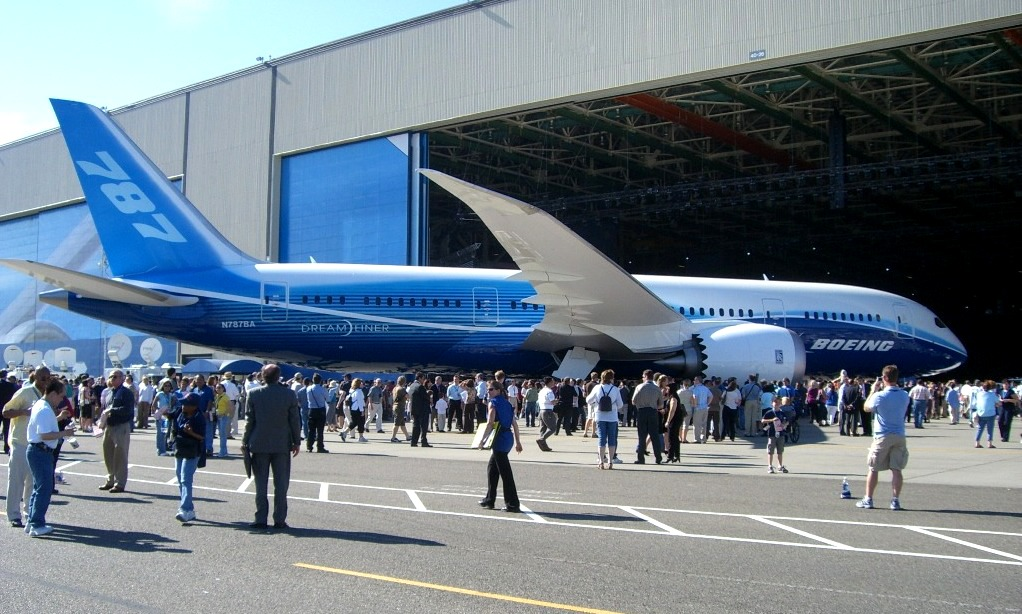
\includegraphics[width=\paperwidth]{dreamliner}};
    \uncover<2->{\node [below right=1cm of dreamliner.north west, anchor=north west]
      {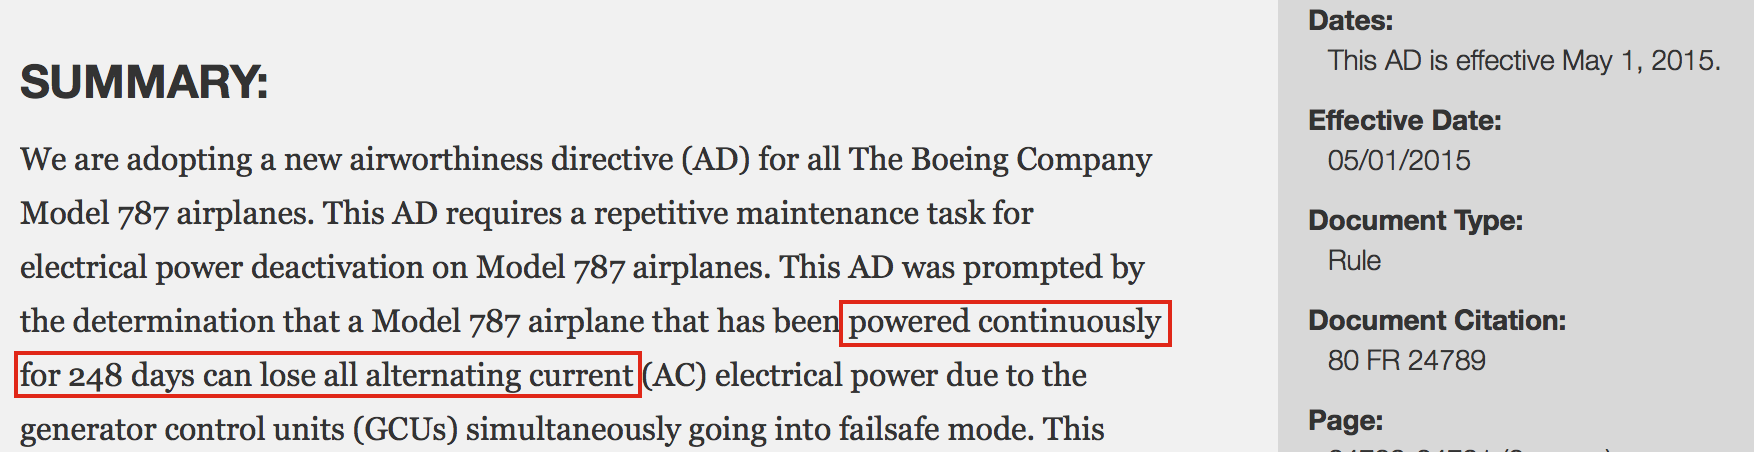
\includegraphics[width=1\framewidth]{dreamliner-bug-2015}};}
    \uncover<3->{\node [above left=1cm of dreamliner.south east, anchor=south east]
      {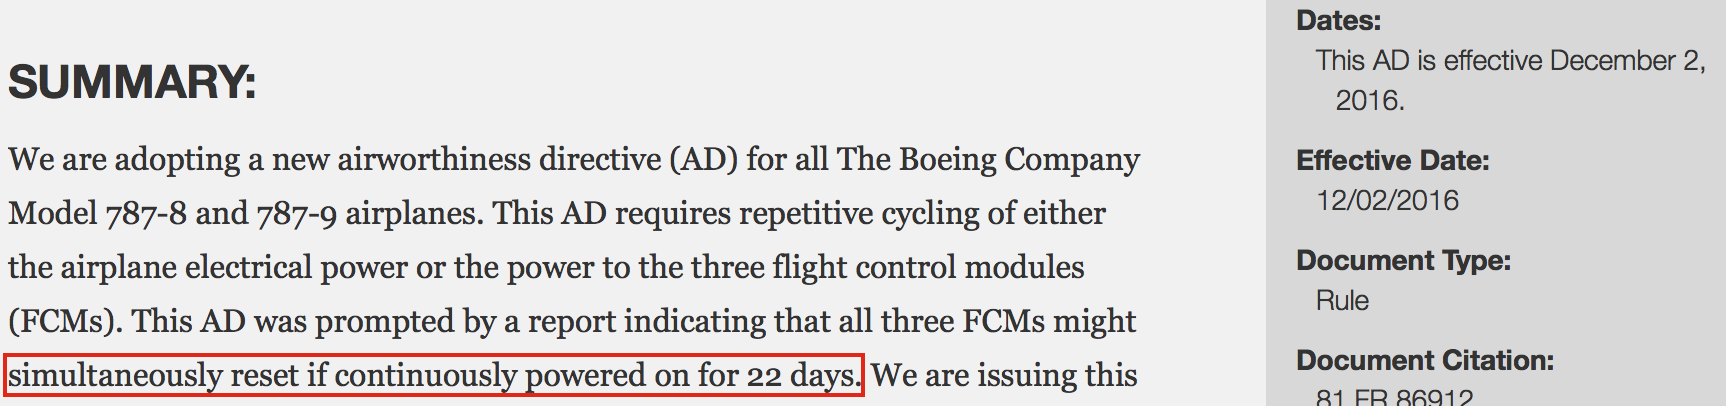
\includegraphics[width=1\framewidth]{dreamliner-bug-2016}};}
  \end{tikzpicture}
\end{frame}

\begin{frame}[fragile]
  \frametitle{The pernicious \texttt{int}}
  Integers are represented either \emph{signed} or \emph{unsigned}
  using a fixed number of \emph{bits}.

  Let's try computing $127+1$, represented as 8bit signed integers.

  \begin{uncoverenv}<2>
  \begin{tikzpicture}
    \matrix (m) [matrix of nodes,
    nodes={minimum size=0.75cm, draw, anchor=center},
    column sep=0pt,
    ]
    { $-2^7$ & $2^6$ & $2^5$ & $2^4$ & $2^3$ & $2^2$ & $2^1$ & $2^0$
      \\};
    \matrix (mfull) [matrix of nodes, below=0.2cm of m,
    nodes={minimum size=0.75cm, draw, anchor=center},
    column sep=0pt,
    ]
    { $0$ & $1$ & $1$ & $1$ & $1$ & $1$ & $1$ & $1$
      \\};
    \node [left=0.1cm of mfull]  {$127$};
    \matrix (mone) [matrix of nodes, below=0.2cm of mfull,
    nodes={minimum size=0.75cm, draw, anchor=center},
    column sep=0pt,
    ]
    { $0$ & $0$ & $0$ & $0$ & $0$ & $0$ & $0$ & $1$
      \\};
    \node [left=0.1cm of mone] {$1$};
    \node [above left=0.1cm and 0.3cm of mone.north west, anchor=center] {$+$};

    \matrix (moops) [matrix of nodes, below=0.2cm of mone,
    nodes={minimum size=0.75cm, draw, anchor=center},
    column sep=0pt,
    ]
    { $1$ & $0$ & $0$ & $0$ & $0$ & $0$ & $0$ & $0$
      \\};
    \node [left=0.1cm of moops] {$-128$};
    \node [above left=0.1cm and 0.3cm of moops.north west, anchor=center] {$=$};
  \end{tikzpicture}
  \end{uncoverenv}
\end{frame}

\begin{frame}[fragile]
  \frametitle{The pernicious \texttt{int}}
  Let's go back and look at the Dreamliner numbers again.

  \begin{equation*}
    248\,\text{days} = 248 \times 24 \times 3600 \times 100 =
    2142720000 \,\text{centiseconds}
  \end{equation*}
  \begin{equation*}
    22\,\text{days} = 22 \times 24 \times 3600 \times 1000 =
    1900800000 \,\text{milliseconds}
  \end{equation*}


  \begin{uncoverenv}<2>
    \begin{equation*}
      \log_2{2142720000} \approx 30.997
    \end{equation*}
  \begin{equation*}
    \log_2{1900800000} \approx 30.824
  \end{equation*}

  Both of these failures are almost certainly due to \emph{integer
    overflow} of a signed 32bit integer.
\end{uncoverenv}
\end{frame}

\begin{frame}[plain,t]
  \begin{flushright}
    \tiny \url{https://cve.mitre.org/cgi-bin/cvekey.cgi?keyword=integer+overflow}
  \end{flushright}
  \begin{tikzpicture}[remember picture, overlay]
    \node[at=(current page.center)]
    {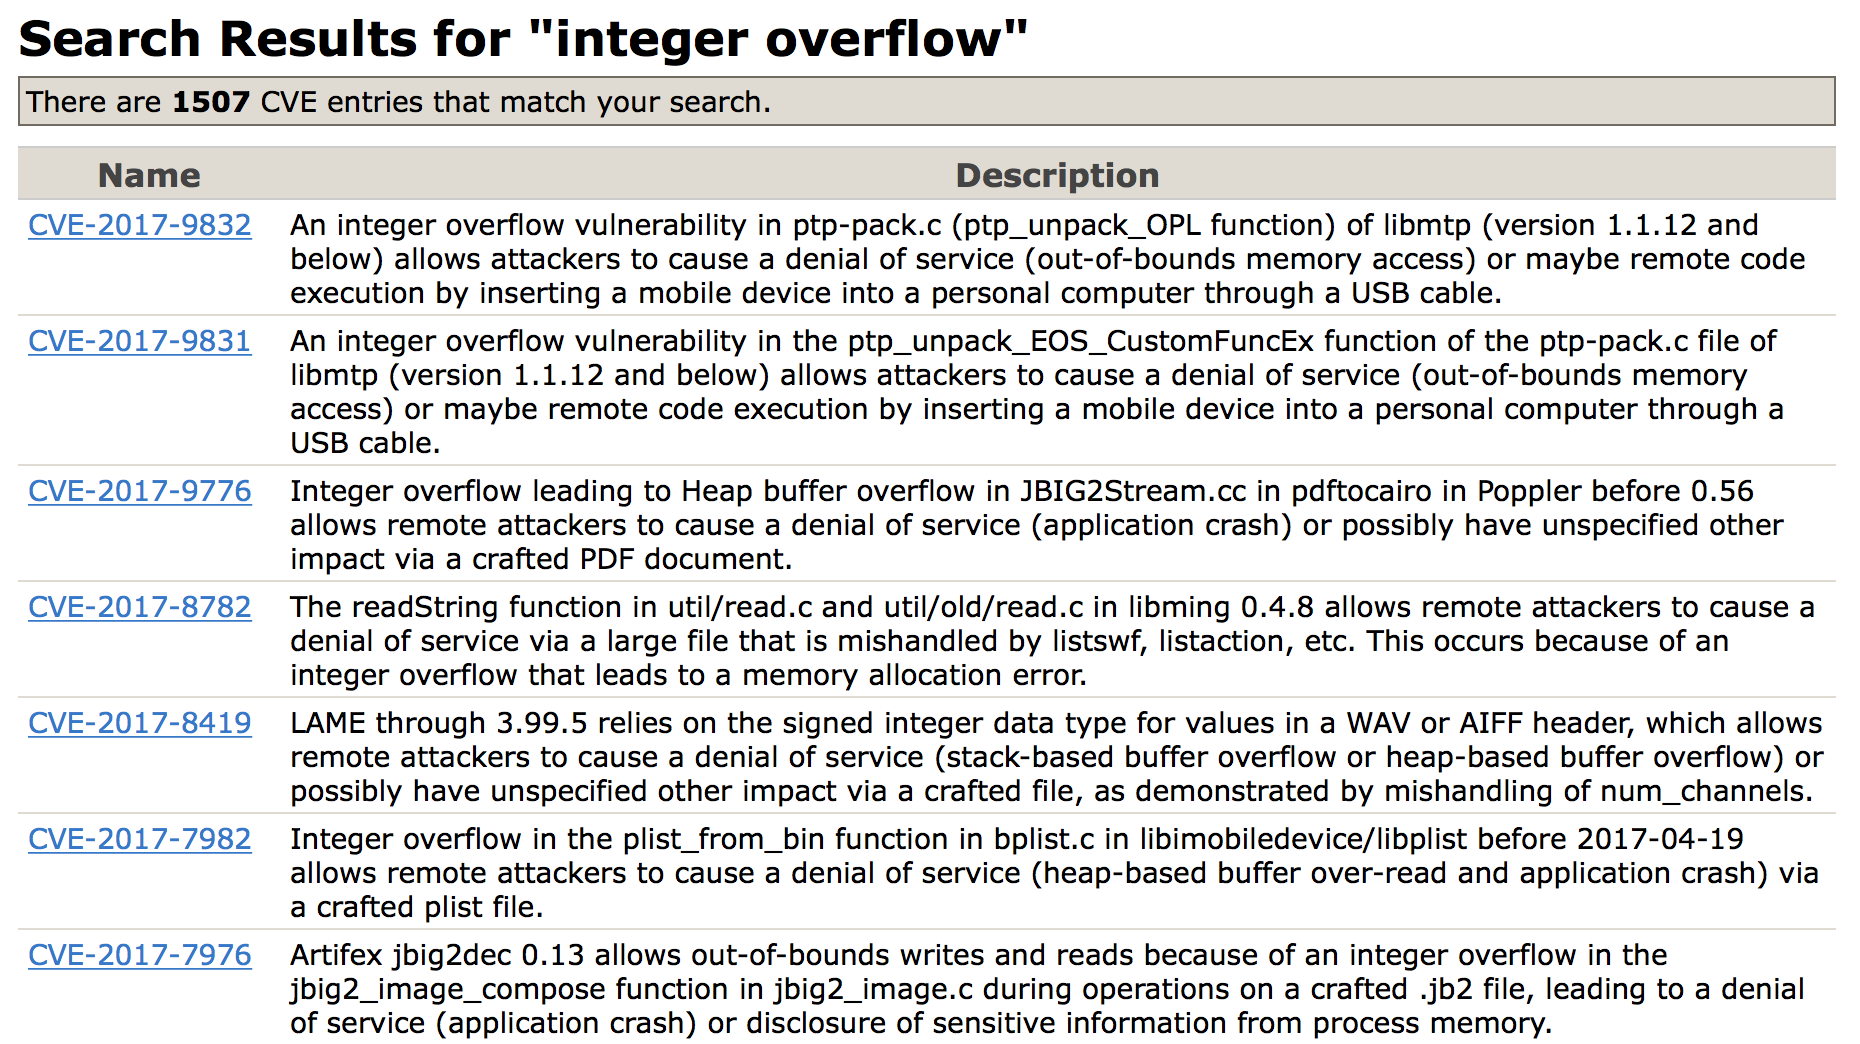
\includegraphics[width=\paperwidth]{cve-overflow}};
  \end{tikzpicture}
\end{frame}

\begin{frame}
  \frametitle{Should you trust your calculation?}

  Computing with real values provides a whole new class of ways to get
  the wrong answer.

  \begin{center}
    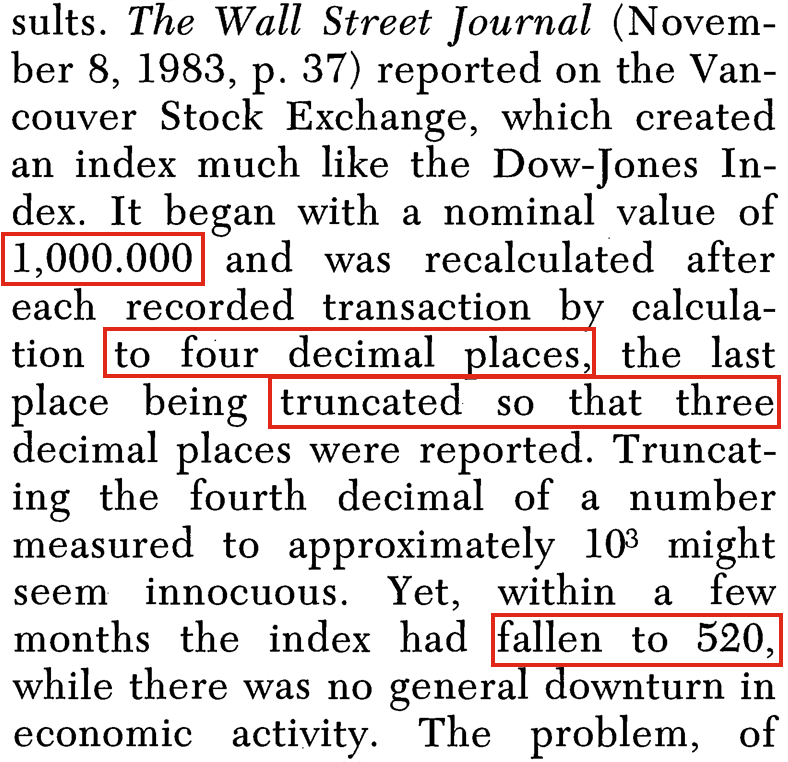
\includegraphics[height=0.6\textheight]{vancouver-index}
  \end{center}
  \begin{flushright}
    \tiny McCullogh \& Vinod, Journal of Economic Literature
    37(2):633--665 (1999)
  \end{flushright}
\end{frame}

\begin{frame}
  \frametitle{Floating point}
  \begin{itemize}
  \item Represent a number as $\alpha \times 10^\beta$.  $\alpha$ the
    \emph{significand} or \emph{mantissa}; $\beta$ the
    \emph{exponent}.
  \item \emph{Floating} because the value of the exponent tells us
    where in the mantissa the decimal point is.
  \item Can only use a \emph{finite} amount of memory for each number,
    which destroys our intuition about how arithmetic behaves.
  \item I will show a few simple examples to rebuild some of that intuition.
  \end{itemize}
\end{frame}
\begin{frame}[fragile]
  \frametitle{No associativity}
  We expect that arithmetic operations \emph{associate}
  \begin{equation*}
    (a + b) - c = a + (b - c).
  \end{equation*}

  Floating point operations do not.

  \begin{center}
    \begin{onlyenv}<2>
\begin{minted}[fontsize=\small]{c}
float a = 1f;
float b = 1e10f;
print ((a + b) - b);
print (a + (b - b));
\end{minted}
    \end{onlyenv}
  \end{center}
  \begin{center}
    \begin{onlyenv}<3>
\begin{minted}[fontsize=\small]{c}
float a = 1f;
float b = 1e10f;
print ((a + b) - b); => 0.0
print (a + (b - b)); => 1.0
\end{minted}
    \end{onlyenv}
  \end{center}
\end{frame}

\begin{frame}[fragile]
  \frametitle{Just add more precision, no?}

  \begin{itemize}
  \item a \emph{single precision} \texttt{float} has about 8 decimal
    digits of precision.
  \item So $1\times10^{10} + 1 = 1\times10^{10} + 0.000,000,000,1\times10^{10} = 1$.
  \item We could have used a \emph{double precision} \texttt{double}
    instead (16 decimal digits).
  \item In this case we have enough digits so we end up with
    $1.000,000,000,1\times10^{10}$.
  \item Which suggests we should always calculate in double precision
    for ``more accuracy''.
  \end{itemize}

  \begin{uncoverenv}<2->
    \begin{columns}
      \begin{column}{0.5\textwidth}
        \begin{onlyenv}<2>
\begin{minted}[fontsize=\scriptsize]{c}
int count = 0;
float x = 0;
for (x=0; x<1.0f; x+=1.0f/6.0f)
    count += 1
printf("%d\n", count)
\end{minted}
        \end{onlyenv}
        \begin{onlyenv}<3->
\begin{minted}[fontsize=\scriptsize]{c}
int count = 0;
float x = 0;
for (x=0; x<1.0f; x+=1.0f/6.0f)
    count += 1
printf("%d\n", count) => 6
\end{minted}
        \end{onlyenv}
      \end{column}
      \begin{column}{0.5\textwidth}
        \begin{onlyenv}<2-3>
\begin{minted}[fontsize=\scriptsize]{c}
int count = 0;
double x = 0;
for (x=0; x<1.0; x+=1.0/6.0)
    count += 1
printf("%d\n", count)
\end{minted}
        \end{onlyenv}
        \begin{onlyenv}<4->
\begin{minted}[fontsize=\scriptsize]{c}
int count = 0;
double x = 0;
for (x=0; x<1.0; x+=1.0/6.0)
    count += 1
printf("%d\n", count) => 7
\end{minted}
        \end{onlyenv}
      \end{column}
    \end{columns}
  \end{uncoverenv}
\end{frame}
\end{document}
